% English translation of chapter1.tex, lines 267--567.
% Source: Methods of Algebra, Volume 2, commit
% 9a5803ff77dd3257484cb177f851a73770a59dd3 (CC BY 4.0).
% stable-unit-id: o014.aljabr2.chapter1.additive-categories-kernels-cokernels

% segment-id: o014.li2.chapter1.additive-categories-kernels-cokernels.h001
\section{Additive Categories: Kernels and Cokernels}\label{sec:Ker-Coker}
\hypertarget{o014.aljabr2.chapter1.additive-categories-kernels-cokernels}{ }

% segment-id: o014.li2.chapter1.additive-categories-kernels-cokernels.p001
This section uses the notion of a functor preserving $\varinjlim$ or $\varprojlim$. This is basic category theory; see \cite[Definition~2.8.8]{Li1} or the brief review in Section~\sourcecrossref{sec:limit-functor}{1.5}. We first recall $\cate{Ab}$-categories and additive categories; see \cite[\S~3.4]{Li1}.

% segment-id: o014.li2.chapter1.additive-categories-kernels-cokernels.l001
\begin{itemize}
	% segment-id: o014.li2.chapter1.additive-categories-kernels-cokernels.i001
	\item A category $\mathcal C$ is an \emph{$\cate{Ab}$-category}, or a \emph{preadditive category}, if every $\Hom(X,Y)$ is an abelian group, written additively (equivalently, a $\Z$-module), and every composition map $\Hom(Y,Z)\times\Hom(X,Y)\to\Hom(X,Z)$ is $\Z$-bilinear. One may therefore speak of the morphism $0\in\Hom(X,Y)$. An $\cate{Ab}$-category may have $\cate{Ab}$-subcategories; every full subcategory is automatically one.
	\index{category!$\cate{Ab}$-}

	% segment-id: o014.li2.chapter1.additive-categories-kernels-cokernels.i002
	\item If $\mathcal C_1,\mathcal C_2$ are $\cate{Ab}$-categories, a functor $F:\mathcal C_1\to\mathcal C_2$ is \emph{additive} if the induced maps on $\Hom$ sets are group homomorphisms. Equivalences of $\cate{Ab}$-categories and their quasi-inverses are always understood to be additive.
	\index{functor!additive}
\end{itemize}

% segment-id: o014.li2.chapter1.additive-categories-kernels-cokernels.p002
We shall need the following elementary but fundamental observation. By convention, a linear map of $\Z$-modules means a module homomorphism.

% segment-id: o014.li2.chapter1.additive-categories-kernels-cokernels.pr001
\begin{proposition}\label{prop:automatic-Ab-morphism}
	Let $\mathcal C$ and $\mathcal C'$ be $\cate{Ab}$-categories.
	% segment-id: o014.li2.chapter1.additive-categories-kernels-cokernels.l002
	\begin{enumerate}
		% segment-id: o014.li2.chapter1.additive-categories-kernels-cokernels.i003
		\item Given adjoint functors
		% segment-id: o014.li2.chapter1.additive-categories-kernels-cokernels.g001
		\[\begin{tikzcd}
			F: \mathcal{C} \arrow[shift left, r] & \mathcal{C}' \arrow[shift left, l] : G
		\end{tikzcd},\]
		with $F,G$ additive, the adjunction isomorphism $\varphi:\Hom_{\mathcal C'}(F(\cdot),\cdot)\rightiso\Hom_{\mathcal C}(\cdot,G(\cdot))$ is linear.
		% segment-id: o014.li2.chapter1.additive-categories-kernels-cokernels.i004
		\item For any $\alpha:I\to\mathcal C$, the isomorphism in the universal property
		% segment-id: o014.li2.chapter1.additive-categories-kernels-cokernels.q001
		\[ \Hom_{\mathcal{C}}\left( \varinjlim \alpha, T \right) \simeq
		\varprojlim_{i \in \Obj(I)} \Hom_{\mathcal{C}}(\alpha(i), T),
		\quad T \in \Obj(\mathcal{C}) \]
		is linear whenever the colimit exists. The analogous assertion holds for $\varprojlim$.
	\end{enumerate}
\end{proposition}

% segment-id: o014.li2.chapter1.additive-categories-kernels-cokernels.pf001
\begin{proof}
	For (i), the discussion following \cite[Definition~2.6.3]{Li1} says that $\varphi$ is determined by the unit $\eta$ and counit $\varepsilon$:
	% segment-id: o014.li2.chapter1.additive-categories-kernels-cokernels.q002
	\[ \varphi(f) = Gf \circ \eta_X, \quad
	\varphi^{-1}(g) = \varepsilon_Y \circ Fg, \quad
	f \in \Hom_{\mathcal{C}'}(FX, Y), \; g \in \Hom_{\mathcal{C}}(X, GY); \]
	bilinearity of composition makes $\varphi$ linear. For (ii), the isomorphism is described by composition with $\iota_i:\alpha(i)\to\varinjlim\alpha$, so it too is linear.
\end{proof}

% segment-id: o014.li2.chapter1.additive-categories-kernels-cokernels.p003
In an $\cate{Ab}$-category, $X_1\times X_2$ exists if and only if $X_1\sqcup X_2$ exists, and then there is a canonical isomorphism $X_1\sqcup X_2\rightiso X_1\times X_2$. This structure is called a \emph{biproduct}; see \cite[Definition~3.4.8, Theorem~3.4.9]{Li1}.
\index{biproduct}

% segment-id: o014.li2.chapter1.additive-categories-kernels-cokernels.p004
More generally, a biproduct of $X_1,\ldots,X_n$ is an object $Z$ with morphisms
% segment-id: o014.li2.chapter1.additive-categories-kernels-cokernels.g002
$\begin{tikzcd} X_i \arrow[r, yshift=-0.5ex, "\iota_i"'] & Z \arrow[l, yshift=0.5ex, "p_i"'] \end{tikzcd}$,
$i=1,\ldots,n$, satisfying

% segment-id: o014.li2.chapter1.additive-categories-kernels-cokernels.q003
\begin{equation}\label{eqn:biproduct-identities}\begin{gathered}
	p_i \iota_j = \begin{cases} \identity, & i=j \\ 0, & i \neq j \end{cases} \qquad
	\sum_{i=1}^n \iota_i p_i = \identity_{Z}.
\end{gathered}\end{equation}

% segment-id: o014.li2.chapter1.additive-categories-kernels-cokernels.p005
Then the families $\iota_i:X_i\to Z$ and $p_i:Z\to X_i$ induce isomorphisms
% segment-id: o014.li2.chapter1.additive-categories-kernels-cokernels.q004
\[ \coprod_{i=1}^n X_i \rightiso Z \rightiso \prod_{i=1}^n X_i. \]
By convention, the biproduct for $n=0$ is a zero object.

% segment-id: o014.li2.chapter1.additive-categories-kernels-cokernels.p006
If an $\cate{Ab}$-category $\mathcal C$ has a zero object, \cite[Lemma~3.4.11]{Li1} ensures that the zero morphism between any $X,Y\in\Obj(\mathcal C)$ agrees with $0\in\Hom(X,Y)$. Moreover, the preceding $\coprod_iX_i\rightiso\prod_iX_i$ is precisely the morphism $\delta$ of \eqref{eqn:coprod-prod-delta}; this follows directly from \eqref{eqn:biproduct-identities}.

% segment-id: o014.li2.chapter1.additive-categories-kernels-cokernels.c001
\begin{convention}\label{con:biproduct}
	\index[sym1]{oplus@$\oplus$}
	Write the $n$-fold biproduct $Z$ as $X_1\oplus\cdots\oplus X_n$. If binary biproducts exist, all $n$-fold biproducts for $n\geq1$ can be formed iteratively using the canonical isomorphism $X_1\oplus X_2\oplus X_3\simeq(X_1\oplus X_2)\oplus X_3$. Also set
	% segment-id: o014.li2.chapter1.additive-categories-kernels-cokernels.q005
	\[ X^{\oplus n} := \underbracket{X \oplus \cdots \oplus X}_{n\; \text{terms}}. \]
	The product diagonal $\delta_X:X\to X^{\oplus n}$ and the coproduct codiagonal $\check\delta_X:X^{\oplus n}\to X$ are characterized by $p_i\delta_X=\identity_X=\check\delta_X\iota_i$ for $1\leq i\leq n$. Explicitly, $\delta_X=\sum_{i=1}^n\iota_i$ and $\check\delta_X=\sum_{i=1}^np_i$.
\end{convention}

% segment-id: o014.li2.chapter1.additive-categories-kernels-cokernels.d001
\begin{definition}[Additive category]\label{def:additive-category}
	\index{category!additive}
	An $\cate{Ab}$-category $\mathcal C$ is \emph{additive} if:
	% segment-id: o014.li2.chapter1.additive-categories-kernels-cokernels.l003
	\begin{compactitem}
		% segment-id: o014.li2.chapter1.additive-categories-kernels-cokernels.i005
		\item it has a zero object $0$;
		% segment-id: o014.li2.chapter1.additive-categories-kernels-cokernels.i006
		\item every two objects $X,Y$ have a biproduct $X\oplus Y$.
	\end{compactitem}
	An $\cate{Ab}$-subcategory of an additive category that is itself additive is an \emph{additive subcategory}. Every finite family $X_1,\ldots,X_n$ in an additive category has a biproduct $X_1\oplus\cdots\oplus X_n$, also called their \emph{direct sum}; the $X_i$ are its direct summands.
	\index{direct sum}
\end{definition}

% segment-id: o014.li2.chapter1.additive-categories-kernels-cokernels.p007
An additive functor $F:\mathcal C_1\to\mathcal C_2$ between additive categories preserves all finite products and coproducts, because:
% segment-id: o014.li2.chapter1.additive-categories-kernels-cokernels.l004
\begin{compactitem}
	% segment-id: o014.li2.chapter1.additive-categories-kernels-cokernels.i007
	\item $F$ preserves biproducts; see \cite[Proposition~3.4.13]{Li1};
	% segment-id: o014.li2.chapter1.additive-categories-kernels-cokernels.i008
	\item $F$ preserves zero objects, since $F(\identity_X)=\identity_{FX}$ and a zero object is characterized by $\identity=0$; see \cite[Lemma~3.4.11]{Li1}.
\end{compactitem}

% segment-id: o014.li2.chapter1.additive-categories-kernels-cokernels.p008
If $\mathcal C$ is an $\cate{Ab}$-category (respectively additive category), then $\mathcal C^{\opp}$ is naturally one as well, with $f\mapsto f^{\opp}$ an isomorphism $\Hom_{\mathcal C^{\opp}}(Y,X)\to\Hom_{\mathcal C}(X,Y)$ of groups.

% segment-id: o014.li2.chapter1.additive-categories-kernels-cokernels.p009
Henceforth, without ambiguity, $0$ denotes both zero objects and zero morphisms in additive categories. A family $f_i:X_i\to X'_i$, $i=1,\ldots,n$, naturally induces $f_1\oplus\cdots\oplus f_n:\bigoplus_iX_i\to\bigoplus_iX'_i$, explicitly $\sum_{i=1}^n\iota'_if_ip_i$.

% segment-id: o014.li2.chapter1.additive-categories-kernels-cokernels.e001
\begin{example}\label{eg:additive-category}
	The category $\cate{Ab}$ is additive: addition on $\Hom$ sets is pointwise, $(f+g)(x)=f(x)+g(x)$; the zero object is the zero group; and biproducts are the usual direct sums. Similarly, $R\dcate{Mod}$ is additive for any ring $R$, and the forgetful functor $R\dcate{Mod}\to\cate{Ab}$ is additive. The category $\cate{Ban}_{\CC}$ of complex Banach spaces and continuous linear maps is also additive. Addition is again pointwise and the zero object is the zero space. For Banach spaces $(X_i,\|\cdot\|_i)$, $i=1,2$, the biproduct may be taken to be the vector-space direct sum $X_1\oplus X_2$ equipped with the norm $\|(x_1,x_2)\|:=\max\{\|x_1\|_1,\|x_2\|_2\}$, where $x_i\in X_i$.
\end{example}

% segment-id: o014.li2.chapter1.additive-categories-kernels-cokernels.pr002
\begin{proposition}\label{prop:additive-cat-addition}
	For morphisms $f,g:X\to Y$ in an additive category $\mathcal C$, $f+g$ is the composite along the top row of the following commutative diagram:
	% segment-id: o014.li2.chapter1.additive-categories-kernels-cokernels.g003
	\[\begin{tikzcd}
		X \arrow[r, "\delta_X"] \arrow[rd] & X \oplus X \arrow[rr, "f \oplus g"] \arrow[d, "\sim" sloped] & & Y \oplus Y \arrow[r, "\check{\delta}_Y"] & Y \\
		& X \times X \arrow[r, "f \times g"] & Y \times Y \arrow[r, "\sim"] & Y \sqcup Y \arrow[ru] \arrow[u, "\sim" sloped] &
	\end{tikzcd}\]
	where $f\times g$ comes from functoriality of products, and $Y\times Y\rightiso Y\sqcup Y$ is the inverse of $\delta$ in \eqref{eqn:coprod-prod-delta}.
\end{proposition}

% segment-id: o014.li2.chapter1.additive-categories-kernels-cokernels.pf002
\begin{proof}
	Write the biproduct maps as $\iota_i^X,\iota_i^Y,p_i^X,p_i^Y$, $i=1,2$. Expressing $\delta_X$ and $\check\delta_Y$ through them verifies the two triangles. Since $f\oplus g=\iota_1^Yfp_1^X+\iota_2^Ygp_2^X$,
	% segment-id: o014.li2.chapter1.additive-categories-kernels-cokernels.q006
	\begin{equation}
		\check{\delta}_Y (f \oplus g) \delta_X = \check{\delta}_Y \iota_1^Y f p^X_1 \delta_X + \check{\delta}_Y \iota_2^Y g p^X_2 \delta_X
		= f + g.
	\end{equation}
	Identifying the biproducts with coproducts, commutativity of the square becomes
	% segment-id: o014.li2.chapter1.additive-categories-kernels-cokernels.g004
	\[\begin{tikzcd}
		X \sqcup X \arrow[r, "{f \sqcup g}"] \arrow[d] & Y \sqcup Y \arrow[d] \\
		X \times X \arrow[r, "{f \times g}"'] & Y \times Y
	\end{tikzcd}\]
	which is precisely functoriality of $\delta$ in \eqref{eqn:coprod-prod-delta}.
\end{proof}

% segment-id: o014.li2.chapter1.additive-categories-kernels-cokernels.co001
\begin{corollary}\label{prop:automatic-additivity}
	Let $\mathcal C,\mathcal C'$ be additive categories and $F:\mathcal C\to\mathcal C'$ a functor.
	% segment-id: o014.li2.chapter1.additive-categories-kernels-cokernels.l005
	\begin{enumerate}[(i)]
		% segment-id: o014.li2.chapter1.additive-categories-kernels-cokernels.i009
		\item $F$ preserves finite products if and only if it preserves finite coproducts.
		% segment-id: o014.li2.chapter1.additive-categories-kernels-cokernels.i010
		\item If $F$ preserves finite products, equivalently finite coproducts, then it is additive.
		% segment-id: o014.li2.chapter1.additive-categories-kernels-cokernels.i011
		\item If $F$ preserves zero objects and biproducts, then it is additive.
		% segment-id: o014.li2.chapter1.additive-categories-kernels-cokernels.i012
		\item If $F$ is an equivalence, then $F$ and its quasi-inverse are additive.
		% segment-id: o014.li2.chapter1.additive-categories-kernels-cokernels.i013
		\item If
		% segment-id: o014.li2.chapter1.additive-categories-kernels-cokernels.g005
		\[\begin{tikzcd}
			F: \mathcal{C} \arrow[shift left, r] & \mathcal{C}' \arrow[shift left, l] : G
		\end{tikzcd}\]
		is an adjoint pair, then $F,G$ are additive; Proposition~\ref{prop:automatic-Ab-morphism} therefore applies.
	\end{enumerate}
\end{corollary}

% segment-id: o014.li2.chapter1.additive-categories-kernels-cokernels.pf003
\begin{proof}
	For (i), a zero object is both the empty product and empty coproduct, so it remains only to consider the product and coproduct of $X,Y$. The canonical isomorphism $\delta:FX\sqcup FY\rightiso FX\times FY$ factors as
	% segment-id: o014.li2.chapter1.additive-categories-kernels-cokernels.q007
	\[ FX \sqcup FY \to F(X \sqcup Y) \rightiso F(X \times Y)
	\to FX \times FY . \]
	For (ii), the composite in Proposition~\ref{prop:additive-cat-addition} along
	% segment-id: o014.li2.chapter1.additive-categories-kernels-cokernels.g006
	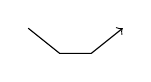
\begin{tikzpicture}[scale=0.4]
		\draw[->] (0, 0.8) -- (1, 0) -- (2, 0) -- (3, 0.8);
	\end{tikzpicture}
	does not use addition on $\Hom$ sets, only finite products and coproducts, the zero object, and their canonical maps. For (iii), all finite products or coproducts are built from zero objects and binary biproducts. Finally, a left adjoint preserves $\varinjlim$, a right adjoint preserves $\varprojlim$ (\cite[Theorem~2.8.12]{Li1}), and equivalences preserve all limits. Thus (iv) and (v) follow from (ii).
\end{proof}

% segment-id: o014.li2.chapter1.additive-categories-kernels-cokernels.p010
In fact, Proposition~\ref{prop:additive-cat-addition} shows that ``additivity'' is a property of the underlying category $\mathcal C$, not additional structure.

% segment-id: o014.li2.chapter1.additive-categories-kernels-cokernels.d002
\begin{definition}
	\index{kernel}\index[sym1]{kerf@$\Ker(f)$}
	\index{cokernel}\index[sym1]{cokerf@$\Coker(f)$}
	Let $\mathcal C$ be an $\cate{Ab}$-category with a zero object, and $f:X\to Y$ a morphism.
	% segment-id: o014.li2.chapter1.additive-categories-kernels-cokernels.l006
	\begin{itemize}
		% segment-id: o014.li2.chapter1.additive-categories-kernels-cokernels.i014
		\item If the equalizer $\Ker(f,0)$ exists, then $\Ker(f):=\Ker(f,0)$ together with $\Ker(f)\hookrightarrow X$ is the \emph{kernel} of $f$.
		% segment-id: o014.li2.chapter1.additive-categories-kernels-cokernels.i015
		\item If the coequalizer $\Coker(f,0)$ exists, then $\Coker(f):=\Coker(f,0)$ together with $Y\twoheadrightarrow\Coker(f)$ is the \emph{cokernel} of $f$.
	\end{itemize}
	Thus the composites $\Ker(f)\to X\to Y$ and $X\to Y\to\Coker(f)$ are both $0$.
\end{definition}

% segment-id: o014.li2.chapter1.additive-categories-kernels-cokernels.p011
Kernels and cokernels admit several complementary viewpoints.
% segment-id: o014.li2.chapter1.additive-categories-kernels-cokernels.l007
\begin{itemize}
	% segment-id: o014.li2.chapter1.additive-categories-kernels-cokernels.i016
	\item For a morphism $g:T\to X$ satisfying $fg=0$,\footnote{Translator's note: the source says ``for every morphism'' without including the condition $fg=0$, or dually $hf=0$. These conditions have been restored because they are precisely the equalizer and coequalizer hypotheses; see correction O014-C006.} the universal property of $\Ker(f)=\Ker(f,0)$ is the commutative diagram
	% segment-id: o014.li2.chapter1.additive-categories-kernels-cokernels.g007
	\[\begin{tikzcd}
		& T \arrow[dashrightarrow, ld, "{\exists! g'}"'] \arrow[d, "g"] \arrow[rd, "0"] & \\
		\Ker(f) \arrow[r] & X \arrow[r, "f"'] & Y .
	\end{tikzcd}\]
	% segment-id: o014.li2.chapter1.additive-categories-kernels-cokernels.i017
	\item For a morphism $h:Y\to T$ satisfying $hf=0$, the universal property of $\Coker(f)=\Coker(f,0)$ is
	% segment-id: o014.li2.chapter1.additive-categories-kernels-cokernels.g008
	\[\begin{tikzcd}
		X \arrow[r, "f"] \arrow[rd, "0"'] & Y \arrow[r] \arrow[d, "h"] & \Coker(f) \arrow[dashrightarrow, ld, "{\exists! h'}"] . \\
		& T &
	\end{tikzcd}\]
	% segment-id: o014.li2.chapter1.additive-categories-kernels-cokernels.i018
	\item The constructions are dual: $\Coker(f)=\Ker(f^{\opp})$ and $\Ker(f)=\Coker(f^{\opp})$.
\end{itemize}

% segment-id: o014.li2.chapter1.additive-categories-kernels-cokernels.p012
Since precisely the zero morphisms factor through a zero object, the universal properties are also characterized by the pullback and pushout diagrams

% segment-id: o014.li2.chapter1.additive-categories-kernels-cokernels.g009
\begin{equation}\label{eqn:Ker-Coker-triangles}
	\begin{tikzcd}
		\Ker(f) \arrow[phantom, r, "\simeq" description] & X \dtimes{Y} 0 \arrow[r] \arrow[d] \arrow[phantom, rd, "\Box" description] & X \arrow[d, "f"] \\
		& 0 \arrow[r] & Y
	\end{tikzcd} \qquad \begin{tikzcd}
		X \arrow[r, "f"] \arrow[d] & Y \arrow[d] & \\
		0 \arrow[r] & Y \dsqcup{X} 0 \arrow[phantom, lu, "\boxplus" description] & \Coker(f) \arrow[phantom, l, "\simeq" description] .
\end{tikzcd}\end{equation}

% segment-id: o014.li2.chapter1.additive-categories-kernels-cokernels.r001
\begin{remark}\label{rem:equalizer-Ker}
	An arbitrary equalizer reduces to a kernel. For
	% segment-id: o014.li2.chapter1.additive-categories-kernels-cokernels.g010
	\[\begin{tikzcd}
	T \arrow[r, "h"] & X \arrow[r, yshift=0.2em, "f"] \arrow[r, yshift=-0.2em, "g"'] & Y
	\end{tikzcd}, \]
	the condition $fh=gh$ is equivalent to $(f-g)h=0$, hence $\Ker(f,g)=\Ker(f-g,0)=:\Ker(f-g)$. Dually, $\Coker(f,g)=\Coker(f-g,0)=:\Coker(f-g)$.
\end{remark}

% segment-id: o014.li2.chapter1.additive-categories-kernels-cokernels.p013
From now on, $\mathcal C$ will mainly be additive.

% segment-id: o014.li2.chapter1.additive-categories-kernels-cokernels.pr003
\begin{proposition}\label{prop:Ker-Coker-composite}
	For morphisms $X\xrightarrow{f}Y\xrightarrow{g}Z$ in an additive category $\mathcal C$, there are commutative diagrams
	% segment-id: o014.li2.chapter1.additive-categories-kernels-cokernels.g011
	\[\begin{tikzcd}[row sep=small, column sep=small]
		\Ker(gf) \arrow[rr, "\sim"] \arrow[hookrightarrow, rd] & & X \dtimes{Y} \Ker(g) \arrow[hookrightarrow, ld] \\
		& X &
	\end{tikzcd} \quad \begin{tikzcd}[row sep=small, column sep=small]
		Z \dsqcup{Y} \Coker(f) \arrow[rr, "\sim"] & & \Coker(gf) \\
		& Z \arrow[twoheadrightarrow, lu] \arrow[twoheadrightarrow, ru] &
	\end{tikzcd}\]
	where $X\dtimes{Y}\Ker(g)\to X$ (respectively $Z\to Z\dsqcup{Y}\Coker(f)$) is the canonical morphism of the fiber product (respectively fiber coproduct),\footnote{Translator's note: the source says ``coproduct,'' but the displayed object is the fiber coproduct $Z\dsqcup{Y}\Coker(f)$ and the proof uses duality with the fiber product; see correction O014-C005.} provided all indicated kernels, cokernels, and limits exist.
\end{proposition}

% segment-id: o014.li2.chapter1.additive-categories-kernels-cokernels.pf004
\begin{proof}
	By \eqref{eqn:Ker-Coker-triangles}, iterated fiber products give canonical isomorphisms $\Ker(gf)\simeq X\dtimes{Z}0\simeq X\dtimes{Y}(Y\dtimes{Z}0)\simeq X\dtimes{Y}\Ker(g)$. Duality gives the cokernel statement.
\end{proof}

% segment-id: o014.li2.chapter1.additive-categories-kernels-cokernels.p014
Functoriality of equalizers and coequalizers induces functoriality of kernels and cokernels, characterized by

% segment-id: o014.li2.chapter1.additive-categories-kernels-cokernels.g012
\begin{equation}\label{eqn:Ker-Coker-functoriality}\begin{tikzcd}
		\Ker(f) \arrow[r] \arrow[dashrightarrow, d, "\exists!"'] & X \arrow[d, "a"'] \arrow[r, "f"] & Y \arrow[d, "b"] \\
		\Ker(g) \arrow[r] & X' \arrow[r, "g"'] & Y'
	\end{tikzcd} \qquad \begin{tikzcd}
		X \arrow[d, "a"'] \arrow[r, "f"] & Y \arrow[d, "b"] \arrow[r] & \Coker(f) \arrow[dashrightarrow, d, "\exists!"'] \\
		X' \arrow[r, "g"'] & Y' \arrow[r] & \Coker(g) .
\end{tikzcd}\end{equation}

% segment-id: o014.li2.chapter1.additive-categories-kernels-cokernels.p015
The next result says that pullback preserves kernels and pushout preserves cokernels.

% segment-id: o014.li2.chapter1.additive-categories-kernels-cokernels.pr004
\begin{proposition}\label{prop:pull-back-ker}
	If
	% segment-id: o014.li2.chapter1.additive-categories-kernels-cokernels.g013
	\[\begin{tikzcd}
		X \arrow[r, "f"] \arrow[d, "a"'] & Y \arrow[d, "b"] \\
		X' \arrow[r, "g"'] & Y'
	\end{tikzcd}\]
	is a pullback (respectively pushout) square in an additive category, then the morphism $\Ker(f)\to\Ker(g)$ (respectively $\Coker(f)\to\Coker(g)$) of \eqref{eqn:Ker-Coker-functoriality} is an isomorphism, provided the indicated objects exist.
\end{proposition}

% segment-id: o014.li2.chapter1.additive-categories-kernels-cokernels.pf005
\begin{proof}
	By duality it suffices to treat pullbacks. For every $T$, the universal properties give canonical isomorphisms
	% segment-id: o014.li2.chapter1.additive-categories-kernels-cokernels.a001
	\begin{align*}
		\Hom(T, \Ker(f)) & \simeq \Ker\left[ \Hom(T, X) \to \Hom(T, Y) \right] \\
		& \simeq \Ker\left[ \Hom(T, Y) \dtimes{\Hom(T, Y')} \Hom(T, X') \to \Hom(T, Y) \right] \\
		& = \Ker\left[ \Hom(T, X') \to \Hom(T, Y') \right] \simeq \Hom(T, \Ker(g)),
	\end{align*}
	and the Yoneda lemma gives $\Ker(f)\rightiso\Ker(g)$; see
	Theorem~\sourcecrossref{prop:Yoneda}{A.1.1}.
\end{proof}

% segment-id: o014.li2.chapter1.additive-categories-kernels-cokernels.lm001
\begin{lemma}\label{prop:mono-epi-ker-coker}
	Let $\mathcal C$ be additive and $f:X\to Y$ a morphism.
	% segment-id: o014.li2.chapter1.additive-categories-kernels-cokernels.l008
	\begin{enumerate}[(i)]
		% segment-id: o014.li2.chapter1.additive-categories-kernels-cokernels.i019
		\item $f$ is monic (respectively epic) if and only if $\Ker(f)=0$ (respectively $\Coker(f)=0$).
		% segment-id: o014.li2.chapter1.additive-categories-kernels-cokernels.i020
		\item $f$ is zero if and only if $\Ker(f)\rightiso X$, equivalently $Y\rightiso\Coker(f)$.
		% segment-id: o014.li2.chapter1.additive-categories-kernels-cokernels.i021
		\item Given $k:Y\to Z$ (respectively $k':W\to X$), there is a unique morphism making the corresponding diagram commute:
		% segment-id: o014.li2.chapter1.additive-categories-kernels-cokernels.g014
		\[\begin{tikzcd}[row sep=small, column sep=small]
		\Ker(kf) \arrow[rd] & & \Ker(f) \arrow[ld] \arrow[hookrightarrow, ll, "\exists !"'] \\
		& X &
		\end{tikzcd} \quad \text{or} \quad
		\begin{tikzcd}[row sep=small, column sep=small]
		\Coker(fk') \arrow[twoheadrightarrow, rr, "\exists !"] & & \Coker(f) \\
		& Y \arrow[lu] \arrow[ru] &
		\end{tikzcd}\]
		provided the indicated kernels or cokernels exist. If $k$ is monic (respectively $k'$ is epic), then $\Ker(f)\rightiso\Ker(kf)$ (respectively $\Coker(fk')\rightiso\Coker(f)$).
	\end{enumerate}
\end{lemma}

% segment-id: o014.li2.chapter1.additive-categories-kernels-cokernels.pf006
\begin{proof}
	For (i), by duality consider only monomorphisms. By definition, $f$ is monic precisely when $f(g_1-g_2)=0\iff g_1-g_2=0$ for every $g_1,g_2:T\to X$. Equivalently, every $g:T\to X$ with $fg=0$ factors through $T\to0\to X$, exactly the universal property of $\Ker(f)=0$. For (ii), $f=0\iff\Ker(f,0)\rightiso X$ follows from the definition of an equalizer. For (iii), use
	% segment-id: o014.li2.chapter1.additive-categories-kernels-cokernels.g015
	\[\begin{tikzcd}[column sep=small]
		\left\{ g \in \Hom(T, X): fg=0 \right\} \arrow[phantom, r, "\subset" description] & \left\{ g \in \Hom(T, X): kfg=0 \right\} \\
		\Hom(T, \Ker(f)) \arrow[u, "1:1"] & \Hom(T, \Ker(kf)) \arrow[u, "1:1"']
	\end{tikzcd}\]
	The top inclusion is equality when $k$ is monic. Apply the Yoneda lemma.
\end{proof}

% segment-id: o014.li2.chapter1.additive-categories-kernels-cokernels.p016
In an additive category, the image and coimage of Definition~\ref{def:Im-Coim} have simple descriptions.

% segment-id: o014.li2.chapter1.additive-categories-kernels-cokernels.pr005
\begin{proposition}\label{prop:Im-Coim-additive}
	\index{image}\index{coimage}
	\index[sym1]{imf@$\Image(f)$}\index[sym1]{coimf@$\Coim(f)$}
	For $f:X\to Y$ in an additive category $\mathcal C$, there are canonical isomorphisms
	% segment-id: o014.li2.chapter1.additive-categories-kernels-cokernels.a002
	\begin{align*}
		\Image(f) & \simeq \Ker\left[ Y \to \Coker(f) \right] \hookrightarrow Y, \\
		\Coim(f) & \simeq \Coker\left[ \Ker(f) \to X \right] \twoheadleftarrow X ;
	\end{align*}
	provided the indicated kernels and cokernels exist.
\end{proposition}

% segment-id: o014.li2.chapter1.additive-categories-kernels-cokernels.pf007
\begin{proof}
	By duality consider only $\Image(f)$. Let $i_1,i_2:Y\to Y\dsqcup{X}Y$ be canonical. By Yoneda it suffices to verify, for every $T$,
	% segment-id: o014.li2.chapter1.additive-categories-kernels-cokernels.q008
	\begin{multline*}
		\Hom\left( T, \Image(f) \right) = \left\{ h: T \to Y \;\middle|\; i_1 h = i_2 h \right\} \\
		= \left\{ \begin{array}{r|l}
			h: T \to Y & \forall S \in \Obj(\mathcal{C}),\; \forall s_1, s_2: Y \to S, \\
			& s_1 f = s_2 f \implies s_1 h = s_2 h
		\end{array}\right\} \\
		\xlongequal{s := s_1 - s_2} \left\{ \begin{array}{r|l}
			h: T \to Y & \forall S \in \Obj(\mathcal{C}),\; \forall s: Y \to S, \\
			& s f = 0 \implies sh = 0
		\end{array}\right\} \\
		= \left\{ \begin{array}{r|l}
			h: T \to Y & T \xrightarrow{h} Y \twoheadrightarrow \Coker(f) \\
			& \text{has composite}\; 0
		\end{array}\right\}
		\leftiso \Hom\left( T, \Ker\left[ Y \to \Coker(f) \right] \right).
	\end{multline*}
	The first equality is $\Image(f):=\Ker(i_1,i_2)$. For the second, rewrite the condition as $s'i_1h=s'i_2h$ for every $s':Y\dsqcup{X}Y\to S$ and use
	% segment-id: o014.li2.chapter1.additive-categories-kernels-cokernels.a003
	\begin{align*}
		\Hom\left( Y \dsqcup{X} Y, S \right) & \xrightarrow{1:1} \Hom(Y,S) \dtimes{\Hom(X,S)} \Hom(Y,S) \\
		s' & \longmapsto \left( s' i_1, s' i_2 \right) =: (s_1, s_2).
	\end{align*}
	The fourth equality follows from the cokernel's universal property, reducing to $S=\Coker(f)$.
\end{proof}

% segment-id: o014.li2.chapter1.additive-categories-kernels-cokernels.p017
If $f=0$, Lemma~\ref{prop:mono-epi-ker-coker}(ii) gives the simplest example: $\Image(f)=0=\Coim(f)$.

% segment-id: o014.li2.chapter1.additive-categories-kernels-cokernels.e002
\begin{example}\label{eg:strict-morphism}
	Continuing Example~\ref{eg:additive-category}, consider $R\dcate{Mod}$. A module homomorphism $f:A\to B$ always has $\Ker(f)=f^{-1}(0)$ and $\Coker(f)=B/\{f(a):a\in A\}$. Its $\Image(f)$ is the set-theoretic image, $\Coim(f)=A/\Ker(f)$, and the comparison in \eqref{eqn:strict-morphism} is the canonical module isomorphism $A/\Ker(f)\rightiso\Image(f)$. Thus every morphism in $R\dcate{Mod}$ is strict.

	Next consider the additive category $\cate{Ban}_{\CC}$ from
	Example~\ref{eg:additive-category}. A continuous linear map $f:X\to Y$ has
	the usual kernel $\Ker(f)=f^{-1}(0)$, which is again a Banach space, while
	$\Coker(f)=Y/\overline{\{f(x):x\in X\}}$ carries the quotient norm. The
	comparison morphism in \eqref{eqn:strict-morphism} becomes
	% segment-id: o014.li2.chapter1.additive-categories-kernels-cokernels.g016
	\[\begin{tikzcd}[row sep=small, column sep=small]
	\Coim(f) \arrow[equal, r] & X/f^{-1}(0) \arrow[r] & \overline{\left\{ f(x): x \in X \right\}} \arrow[equal, r] & \Image(f) \\
	& x + f^{-1}(0) \arrow[mapsto, r] \arrow[phantom, u, "\in" description, sloped] & f(x) \arrow[phantom, u, "\in" description, sloped] &
	\end{tikzcd}\]
	where the right side has the topology induced from $Y$ and the left the quotient topology from $X$. If $f:X\to Y$ is a continuous injective linear map of Banach spaces with dense, non-surjective image, then $\Coim(f)=X\to Y=\Image(f)$ is not an isomorphism. Hence $\cate{Ban}_{\CC}$ has non-strict morphisms.
\end{example}
